\section{Comparison across series of CV models}
\label{sxn:cv}


\michael{Need to say that such large $\alpha$ values don't mean much.}

\michael{Need to highlight difference between $\alpha$ and $\hat{\alpha}$.}


In this section, we examine the quality metrics described in Section~\ref{sxn:methods} for several CV model architecture series.
This includes the VGG, ResNet, and DenseNet series of models, each of which consists of several pretrained DNN models, trained on the full ImageNet~\cite{imagenet} dataset, and each of which is distributed with the current opensource pyTorch framework (version 1.4)~\cite{pyTorch}.
This also includes results for a larger set of ResNet models, trained on the ImageNet-1K dataset~\cite{imagenet1k}, provided on the OSMR ``Sandbox for training convolutional networks for computer vision''~\cite{osmr}, which we call the ResNet-1K series.

We use our quality metrics to perform \emph{coarse model analysis}, comparing and contrasting the three (or four, if ResNet-1K is a distinct series) model series, permitting us to understand the gross properties of these models. 
We also use our metrics to perform \emph{fine layer analysis}, permitting us to understand more fine-scale properties of these models as a function of model depth.


\paragraph{Quality Metrics versus Reported Test Accuracies.}

We have examined the performance of the four quality (Frobenius norm, Spectral norm, Weighted Alpha, and $\alpha$-Norm) applied to each of the VGG, ResNet, ResNet-1K, and DenseNet series.
To start, Figure~\ref{fig:vgg-metrics} plots the four quality metrics versus the reported Test accuracies~\cite{pyTorchVgg}, as well as a basic linear regression line, 
%with the Root Mean Squared Error (RMSE) shown, 
for the pretrained models VGG11, VGG13, VGG16, and VGG19, with and without BatchNormalization.
\michael{These are all log norms, right?}
\michael{XXX.  WHERE IS RMSE.  IN THAT TABLE?}
All four metrics correlate quite well with the reported Top1 Accuracies, with smaller norms and smaller values of $\hat{\alpha}$ implying better generalziation (i.e., greater accuracy, lower error). 
Similar results (not shown) are obtained for the Top5 Accuracies.  
Notice that the log $\alpha$-Norm metric $\log\Vert\mathbf{W}\Vert)_{\infty}^{\infty}$ 
\michael{XXX IS THAT A TYPO} 
performs best, with an RMSE of $0.34$; and the second best metric is $\hat\alpha$, which is an approximate log $\alpha$-Norm metric.
\michael{Are those numbers stale, I don't see them, and some things seem in the other order.}
\charles{See Figure 2}
\michael{We should probably point to the table if we cite quantitative results.}


Figure~\ref{fig:cv2-accuracy} plots the best performing metric ($\alpha$-Norm) for the full ResNet, ResNet-1K, and DenseNet series.
(A much more detailed set of plots---including the behavior of all four metrods on each of the series---are availale at \michael{give web link}.)
For a more visual depiction, Figure~\ref{fig:cv2-accuracy} displays the log $\alpha$-Norm metric  $\log\Vert\mathbf{W}\Vert)_{\infty}^{\infty}$ versus test accuracies for the ResNet, ResNet-1K, and DenseNet series. 
Notice that ResNet series, which has been trained on the full
ImageNet dataset, has an RMSE of $0.66$, whereas the ResNet-1K series, which has been trained on the much smaller ImageNet-1K dataset,
also correlated wells, but has a much larger RMSE of $1.9$.

Table \ref{table:cv-models} summarizes results for all four metrics (Frobenius norm, Spectral norm, Weighted Alpha, and $\alpha$-Norm) applied to the VGG, ResNet, ResNet-1K, and DenseNet series.
\michael{XXX.  AGAIN, WHERE IS RMSE, IN THAT TABLE?}
\charles{The Table may be stale, see the figures to confirm}

For all series, all four metrics correlate quite well with the reported Top1 test accuracies.  
Moreover, the $\alpha$-Norm and/or the approximate Weighted Alpha metrics perform best.


\begin{figure}[t]
    \centering
    \subfigure[ Frobenius Norm, VGG ]{
        %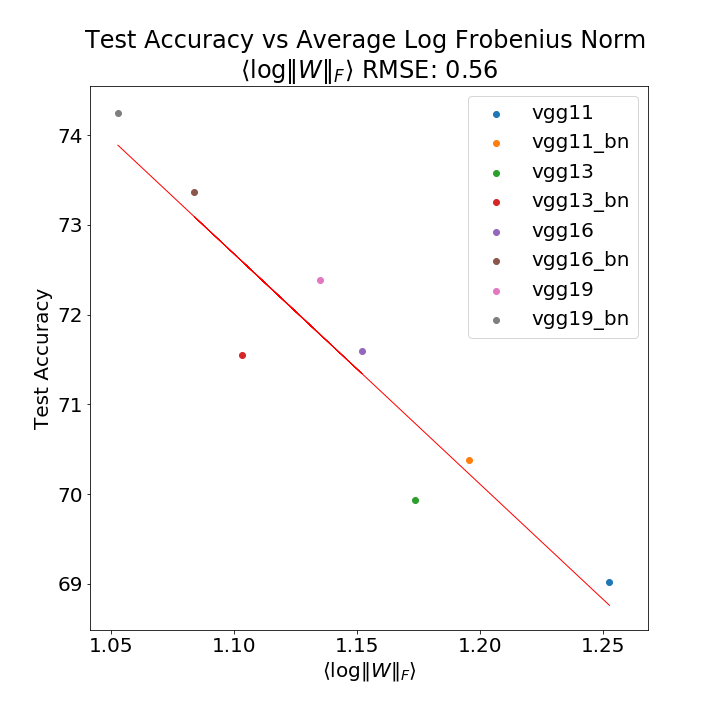
\includegraphics[width=5cm]{img/VGG_lognorm_accs.png}
        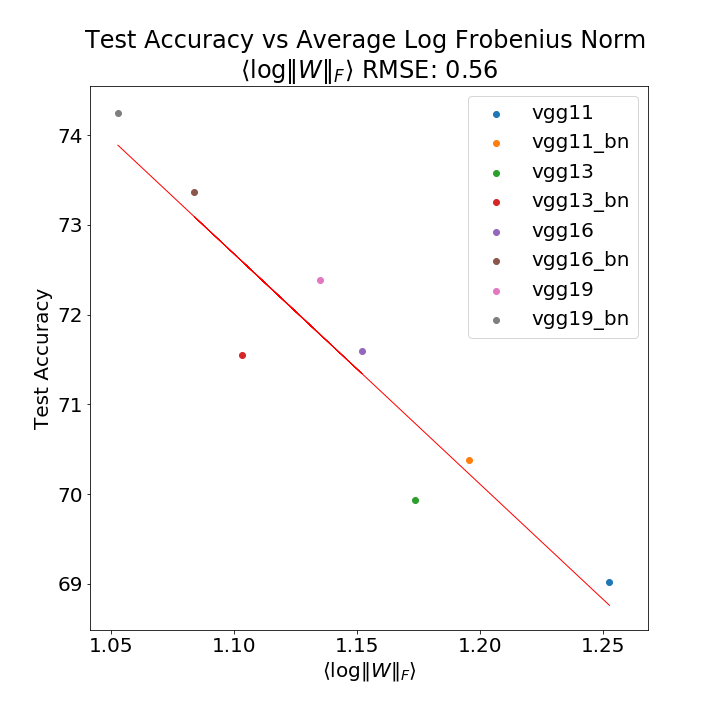
\includegraphics[width=3.7cm]{img/VGG_lognorm_accs.png}
        \label{fig:vgg-fnorm}
    }
    %\qquad
    \subfigure[ Spectral Norm, VGG ]{
        %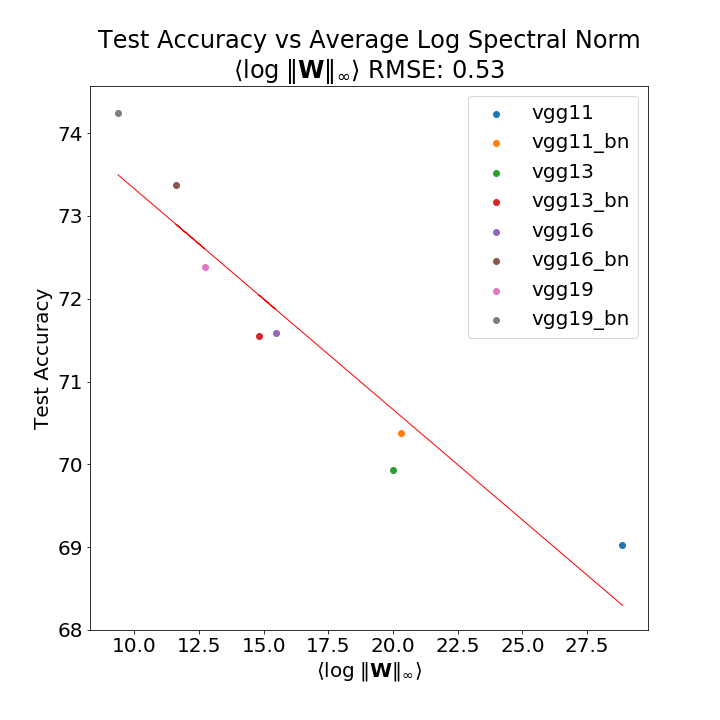
\includegraphics[width=4.9cm]{img/VGG_spectralnorm_accs.png}
        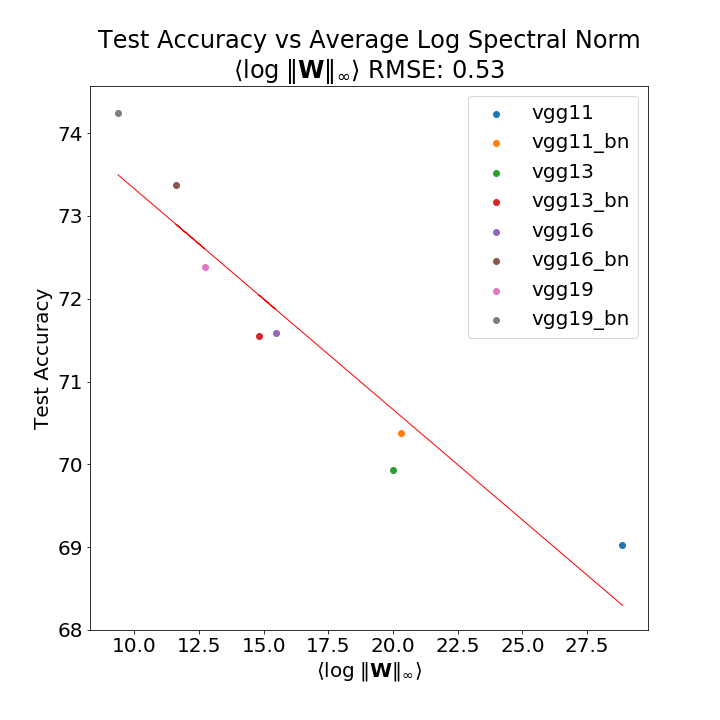
\includegraphics[width=3.7cm]{img/VGG_spectralnorm_accs.png}
        \label{fig:vgg-snorm}
    }
    %\qquad
    \subfigure[ Weighted Alpha, VGG ]{
        %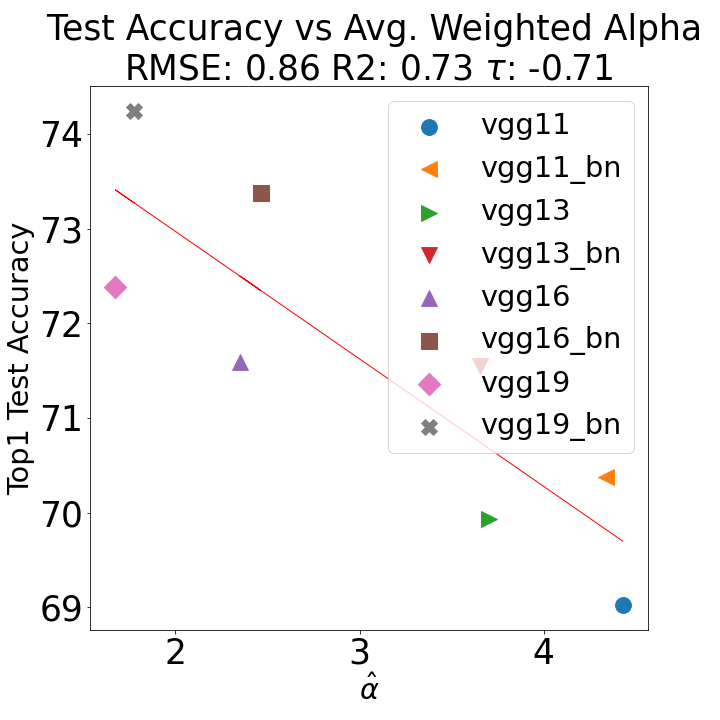
\includegraphics[width=4.9cm]{img/VGG_alpha_weighted_accs.png}
        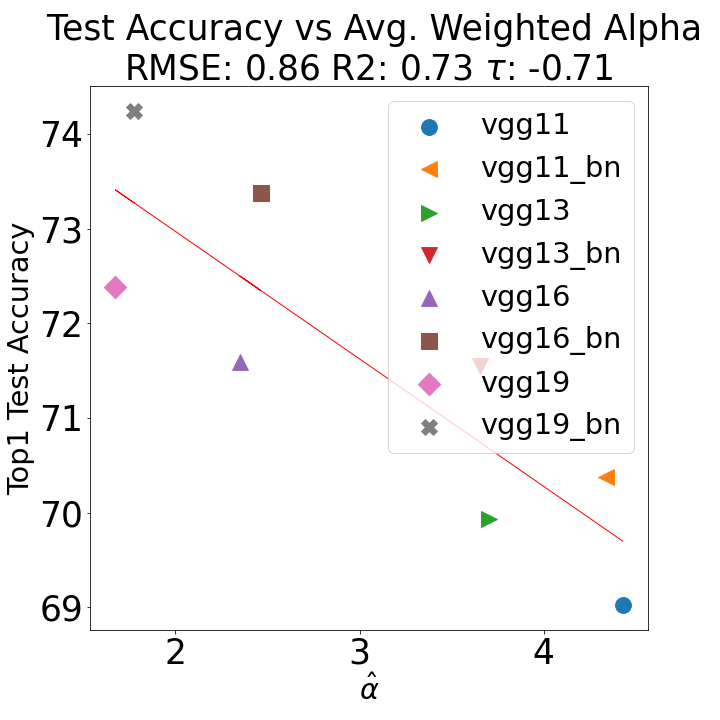
\includegraphics[width=3.7cm]{img/VGG_alpha_weighted_accs.png}
        \label{fig:vgg-walpha}
    }
    %\qquad
    \subfigure[ $\alpha$-Norm, VGG ]{
        %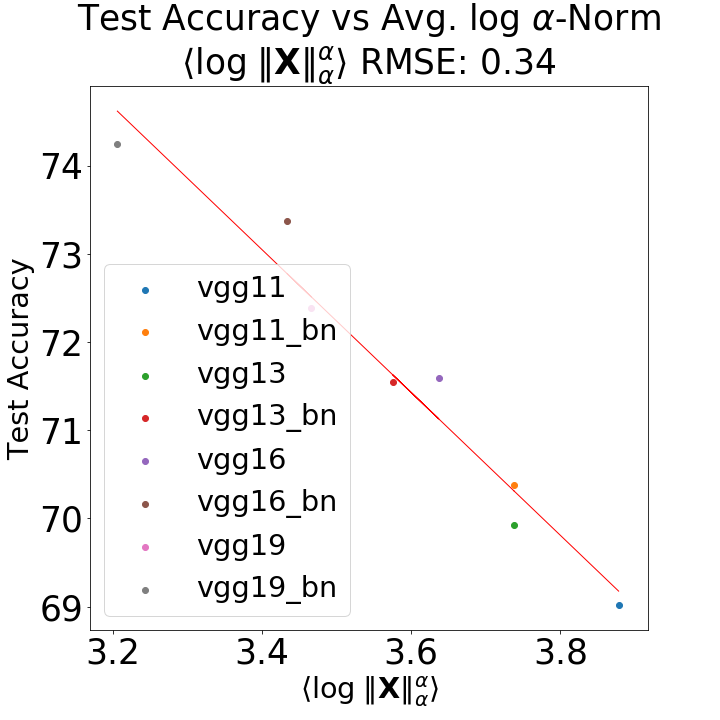
\includegraphics[width=4.9cm]{img/VGG_logpnorm_accs.png}
        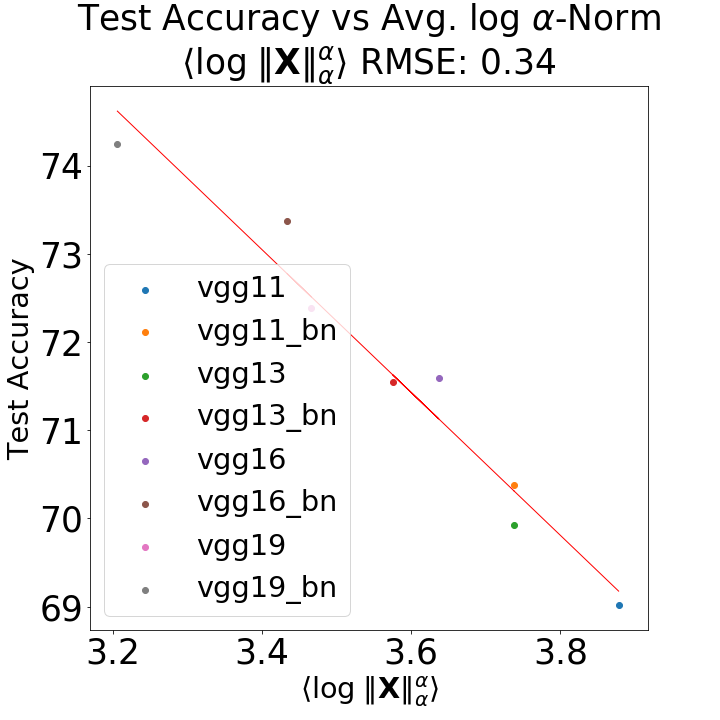
\includegraphics[width=3.7cm]{img/VGG_logpnorm_accs.png}
        \label{fig:vgg-pnorm}
    }
    \caption{Comparison of quality metrics versus reported test accuracy for pretrained VGG models, trained on ImageNet, available in pyTorch.  
             XXX Plots will be updated and replaced. 
             \michael{Figures are unreadable, can we make fonts bigger, etc.}
            }
    \label{fig:vgg-metrics}
\end{figure}


\begin{figure}[t]
    \centering

    \subfigure[ ResNet, $\alpha$-Norm ]{
        %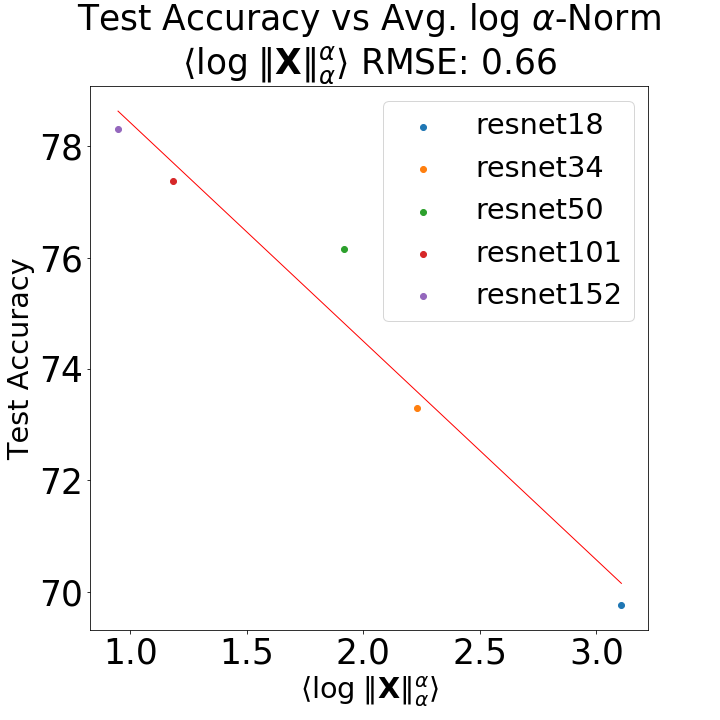
\includegraphics[width=4.2cm]{img/ResNet_logpnorm_accs.png}
        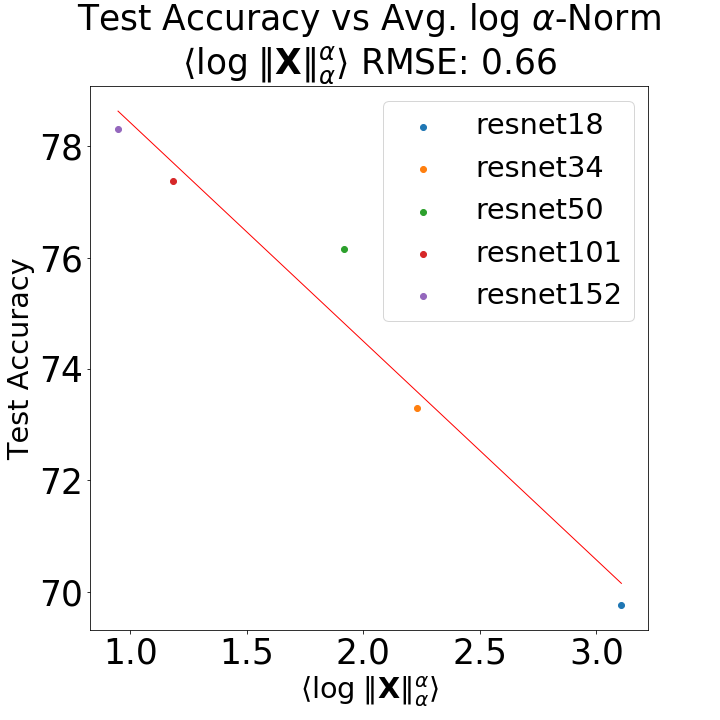
\includegraphics[width=3.7cm]{img/ResNet_logpnorm_accs.png}
        \label{fig:resnet-accuracy}
    }
    \qquad
    \subfigure[ ResNet-1K, $\alpha$-Norm ]{
        %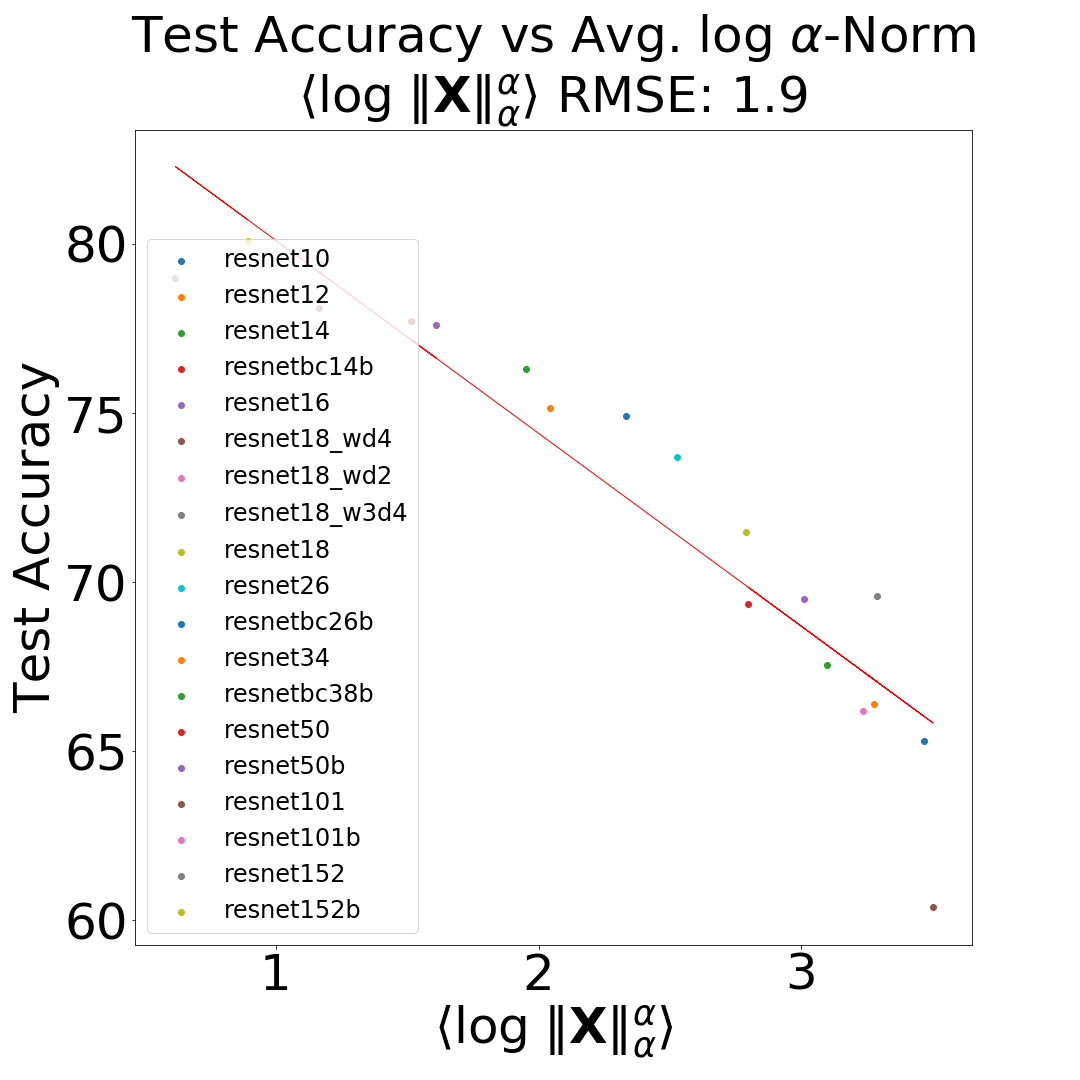
\includegraphics[width=4.5cm]{img/ResNet-1K_logpnorm_accs.png}
        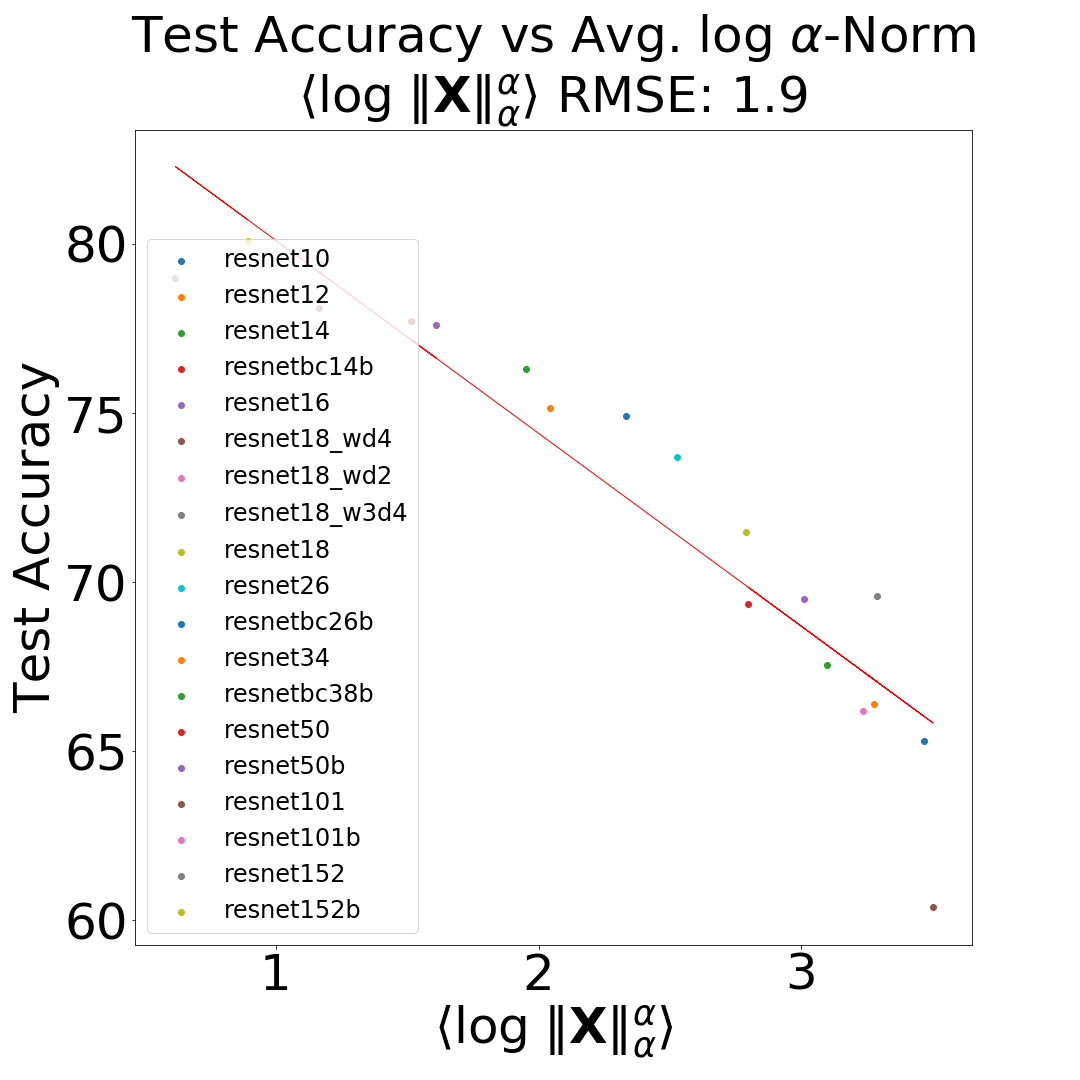
\includegraphics[width=3.7cm]{img/ResNet-1K_logpnorm_accs.png}
        \label{fig:resnet1k-accuracy}
    }
    \qquad
    \subfigure[ DenseNet, $\alpha$-Norm ]{
        %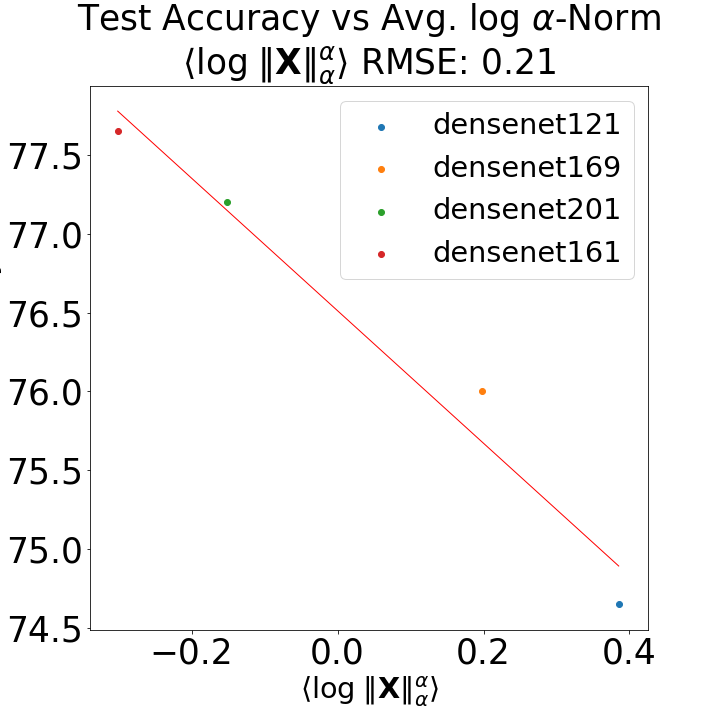
\includegraphics[width=4.4cm]{img/DenseNet_logpnorm_accs.png}
        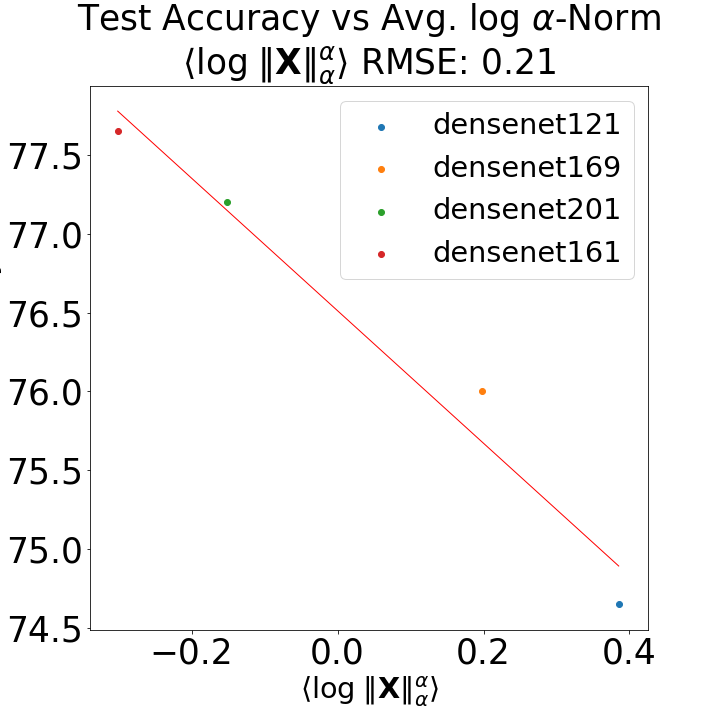
\includegraphics[width=3.7cm]{img/DenseNet_logpnorm_accs.png}
        \label{fig:densenet-accuracy}
    }
    \caption{$\alpha$-Norm versus reported Top1 Error for  ResNet, ResNet-1K, and DenseNet models. The corresponding results for VGG are shown in Figure~\ref{fig:vgg-pnorm}.  }
    \label{fig:cv2-accuracy}
\end{figure}


\begin{table}[t]
\small
\begin{center}
%\begin{tabular}{|p{1in}|c|c|c|c|c|}
\begin{tabular}{|p{0.75in}|c|c|c|c|c|}
%\begin{tabular}{|l|c|c|c|c|c|}
\hline
%   &    & Frobenius Norm & Spectral Norm & Weighted Alpha & Alpha-Norm \\
% Series & \#Models   & $\Vert\mathbf{W}\Vert_{F}$ & $\Vert\mathbf{W}\Vert_{2}$ & $\hat{\alpha}=\alpha\log\lambda_{max}$ & $\Vert\mathbf{X}\Vert^{\alpha}_{\alpha}$ \\
        & Num.   & $\Vert\mathbf{W}\Vert_{F}$ & $\Vert\mathbf{W}\Vert_{2}$ & $\hat{\alpha}$ & $\Vert\mathbf{X}\Vert^{\alpha}_{\alpha}$ \\
 Series & Models & Metric                     & Metric                     & Metric         & Metric                                   \\
\hline
 VGG & 6 & 0.56 & 0.53 & 0.48 & 0.42  \\
 ResNet & 5 & 0.9 & 1.4 & 0.61 & 0.66  \\
 ResNet-1K & 19 & 2.4 & 3.6 & 1.8 & 1.9  \\
 DenseNet & 4 & 0.3 & 0.26 & 0.16 & 0.21 \\
\hline
\end{tabular}
\end{center}
\caption{RMSE (smaller is better) for linear fits of quality metrics to Reported Top1 Test Error for pretrained models in each architecture series.  VGG, ResNet, and DenseNet were pretrained on ImageNet, and ResNet-1K was pretrained on ImageNet-1K. }
\label{table:cv-models}
\end{table}


\paragraph{Layer Analytics: Correlation Flow in CV Models.}

We can learn much more about a pretrained model by going beyond average values to examining quality metrics for each layer weight matrix, $\mathbf{W}$, as a function of depth (or layer id).  % in the network. 
The most interesting results are seen when we plot the PL exponent, $\alpha$, as a function of depth.
%
See Figure~\ref{fig:vgg-alpha-layers}, which plots $\alpha$ for each layer (the first corresponds to data, the last to labels) for the least accurate (shallowest) and most accurate (deepest) model in each of the VGG (without BatchNormalization), ResNet-1K, and DenseNet~series.

\begin{figure}[t]
    \centering

    \subfigure[ VGG ]{
        %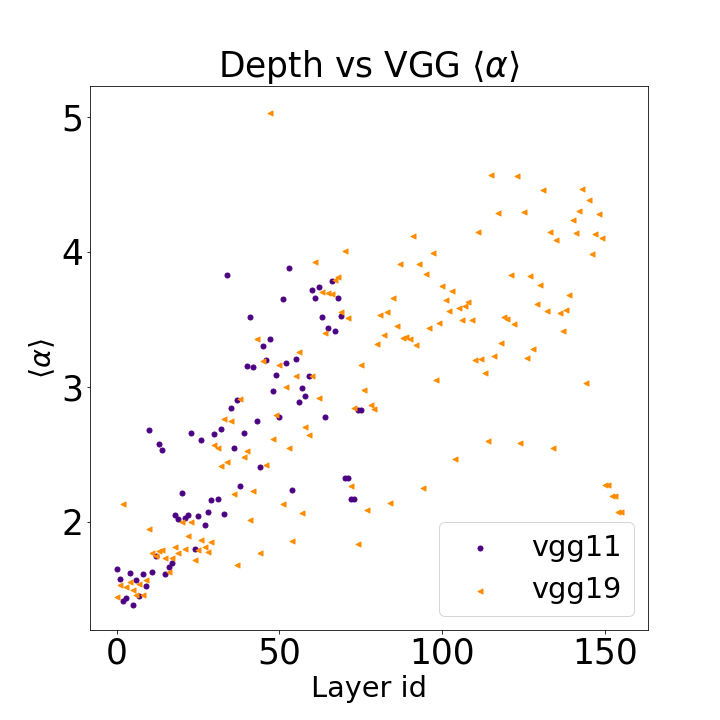
\includegraphics[width=4.5cm]{img/VGG_fnl_alpha_depth.png} 
        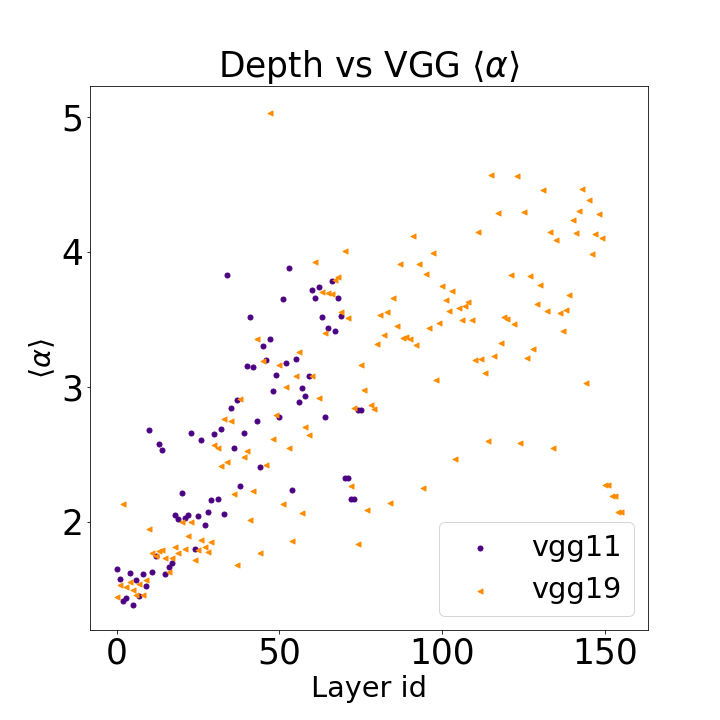
\includegraphics[width=3.7cm]{img/VGG_fnl_alpha_depth.png} 
                \label{fig:vgg-alpha-layers}
    }
    \qquad
    \subfigure[ ResNet-1K ]{
        %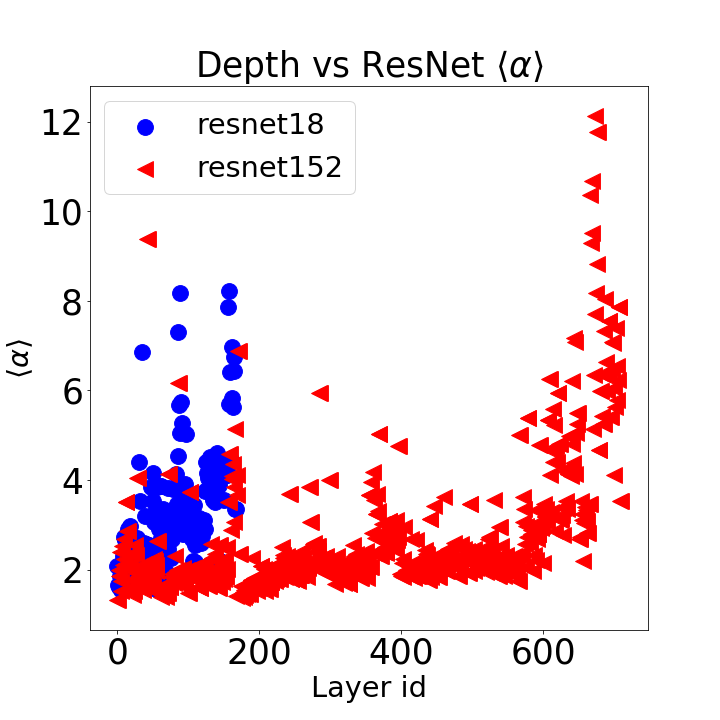
\includegraphics[width=4.5cm]{img/ResNet_fnl_alpha_depth.png} 
        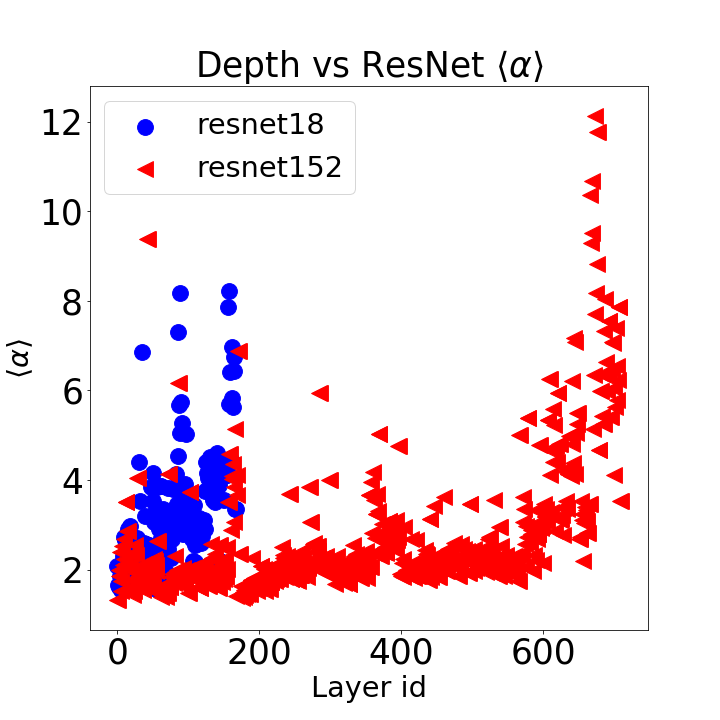
\includegraphics[width=3.7cm]{img/ResNet_fnl_alpha_depth.png} 
        \label{fig:resnet-alpha-layer}
    }
    \qquad
    \subfigure[ DenseNet ]{
        %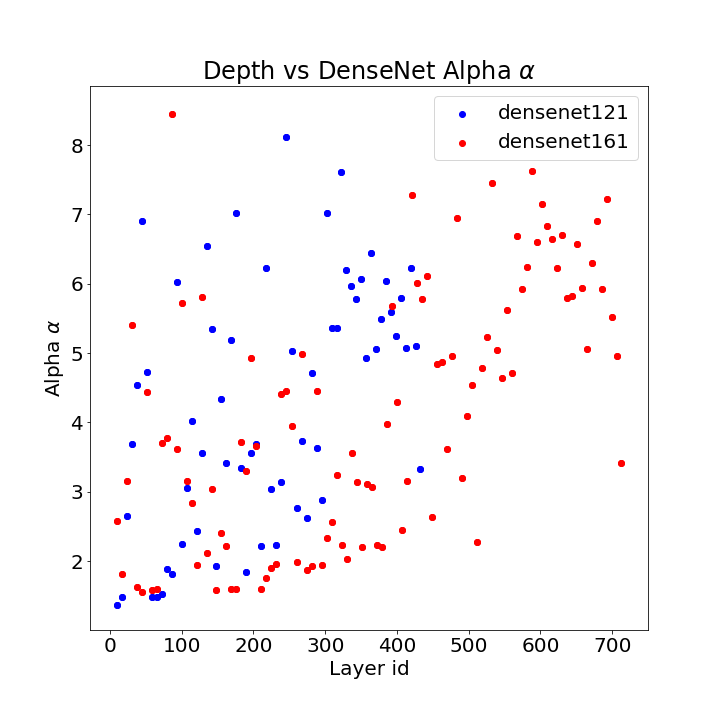
\includegraphics[width=4.5cm]{img/DenseNet_fnl_alpha_depth.png} 
        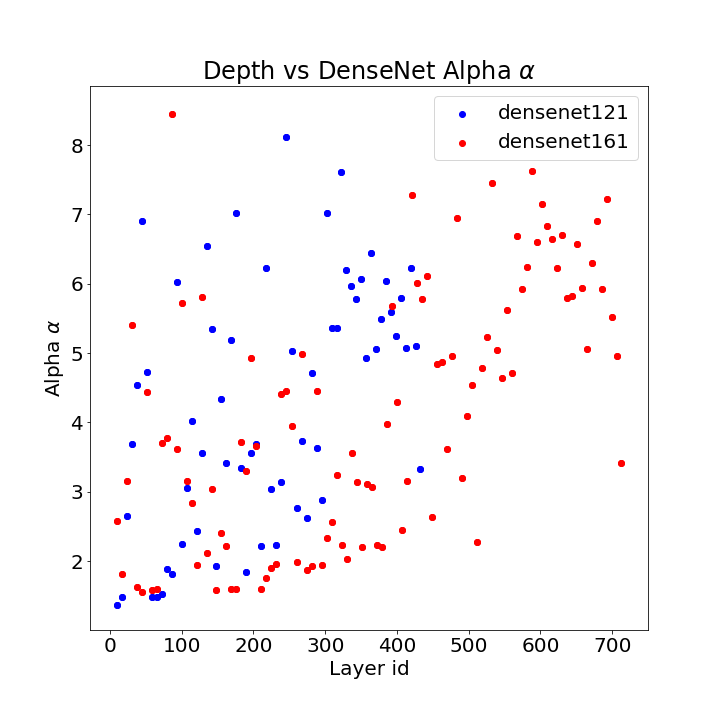
\includegraphics[width=3.7cm]{img/DenseNet_fnl_alpha_depth.png} 
        \label{fig:densenet-alpha-layer}
    }
    \caption{PL exponent $\alpha$ versus layer for VGG, ResNet-1K, and DenseNet models.  Y axes on each plot are different.  ResNet-1K exhibits very different and much more stable behavior across layers, which we interpret in the text as a \emph{correlation flow} across the layers.  }
    \label{fig:vgg-alpha-layers}
\end{figure}

In the VGG models, $\alpha$ systematically increases as we move down the network, from data to labels, in the Conv2D layers, starting with $\alpha\lesssim 2.0$ and reaching all the way to $\alpha\sim 5.0$; and then, in the last three, large, fully-connected (FC) layers, $\alpha$ stabilizes back down to $\alpha\in[2,2.5]$.
This is seen for all the VGG models (again, only the shallowest and deepest are shown in this figure), indicating that the main effect of increasing depth is to increase the range over which $\alpha$ can increase, thus leasing to larger $\alpha$ values in later Conv2D layers of the VGG models.
This is quite different than the behavior of either the ResNet-1K models or the DenseNet models.

For the ResNet-1K models, $\alpha$ also increases in the last few layers, but as the models get deeper, there is a wide range over which $\alpha$ values tend to remain small.
\michael{Can we say something about exceptions which are larger than for VGG or DenseNet.}
\charles{You have the same plots I do..what do you want to say >}
This is seen for other models in the ResNet-1K series, but it is most pronounced for the larger ResNet-1K (152) model, where $\alpha$ remains relatively stable at $\alpha\sim 2.0$, from the earliest layers all the way until we reach close to the final layers.  

For the DenseNet models, $\alpha$ tends to increase as the layer id increases, in particular for layers toward the end.
This is similar to what is seen in the VGG models, but with the DenseNet models, the variance is much larger (in particular for the earlier and middle layers, where it can range all the way to $\alpha\lesssim 8.0$) and much less systematic.

We can understand Figure~\ref{fig:vgg-alpha-layers} in terms of the \emph{flow of correlation}, as follows.
Informally, one would expect a DNN model to perform well when it fascilitates the propagation of information/features across layers.
In the absence of training/test data, we can to try to quantify this by measuring the PL properties of weight matrices.
Smaller $\alpha$ values correspond to layers in which correlations across multiple scales are better captured~\cite{MM18_TR,SornetteBook}, and thus we expect that values of $\alpha$ that are stable across multiple layers enable better \emph{correlation flow} through the network.

Consider the differences---in particular, the number of residual connections---between the VGG, ResNet, and DenseNet architectures.
VGG, while a good model in many ways, was limited by needing a massive FC layers at the end of the model, requiring significant memory and computational resources, and it's poor conditioning led to problems with vanishing gradients.  
The empirical manifestations of this (on weight matrices) are that fitted $\alpha$ values get much worse for deeper layers.
ResNet greatly improved on VGG by introducing residual connections, allowing for greater accurary with far fewer parameters.
(Indeed, ResNet models of up to 1000 layers have been trained.) 
We conjuecture that the effeciency and effectivness of ResNet is reflected in the smaller and more stable $\alpha\sim 2.0$, across nearly all layers, indicating that the inner layers are very well correlated and strongly optimized.
This should also be contrasted with the DenseNet model, which contains many connections between every layer.
Our results (large $\alpha$, meaning they even a HT model is probably a poor fit) suggest that DenseNet has too many connections, diluting the correlation flow across layers, and leaving many layers very poorly optimized.


\paragraph{Layer Analytics: Behavior on Less Thoroughy Studied CV Models.}

Figure~\ref{fig:vgg-metrics} and Table~\ref{table:cv-models} show that---for well-trained and widely-studied models---the weighted $\hat{\alpha}$ metric performs better than but similar to norm-based metrics.
This suggests an obvious question: is the $\hat{\alpha}$ metric just a variation of these more familiar norm-based metrics, or does it capture something different?  
To show that it is not just a variation and that it does capture something different, consider the following less thoroughy studied model, a compressed DNN model~\cite{CWZZ17_TR}, where we observed that the average (Frobenius or Spectral) norm increases with decreasing test error, whereas the average $\alpha$ decreases, as expected.  

\begin{figure}[t]
   \centering
   \subfigure[$\lambda_{max}$ for ResNet20 layers]{
      %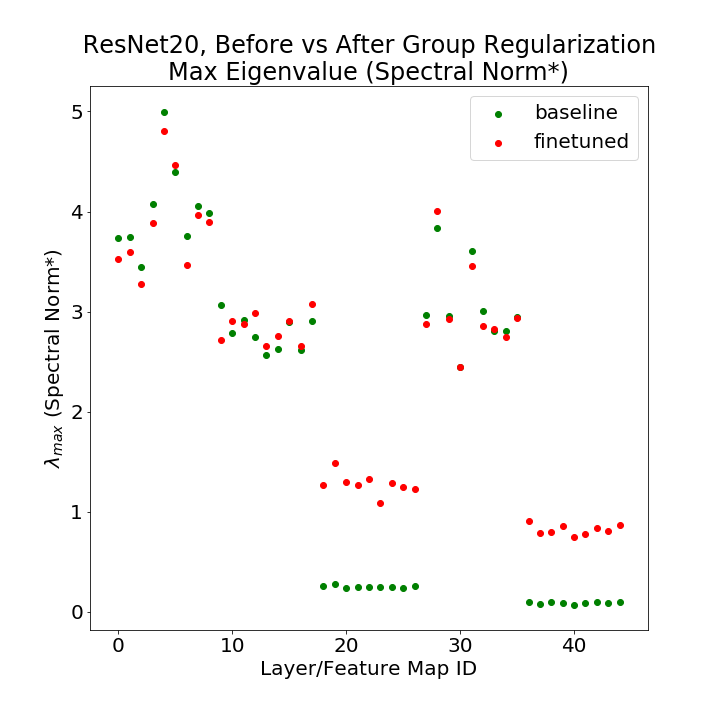
\includegraphics[scale=0.14]{img/resnet4d_maxev.png}
      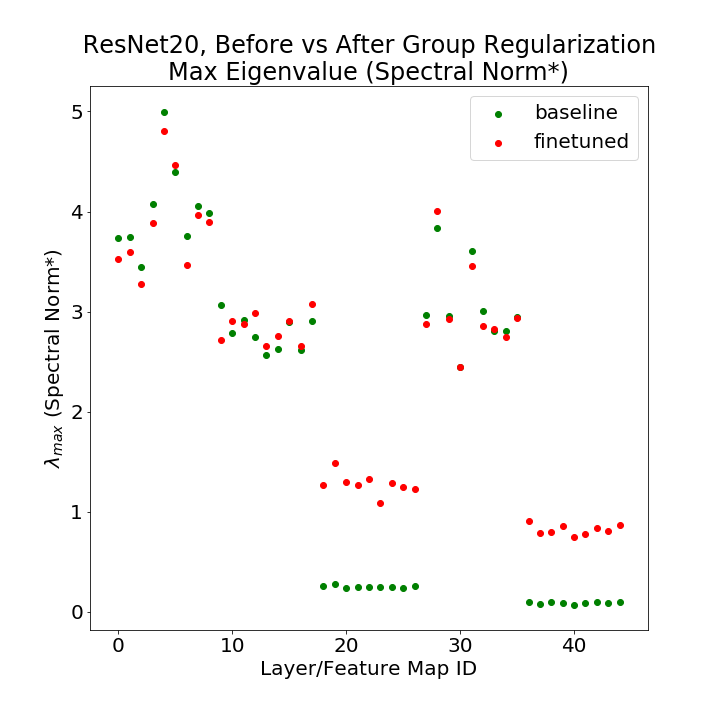
\includegraphics[width=3.7cm]{img/resnet4d_maxev.png}
      %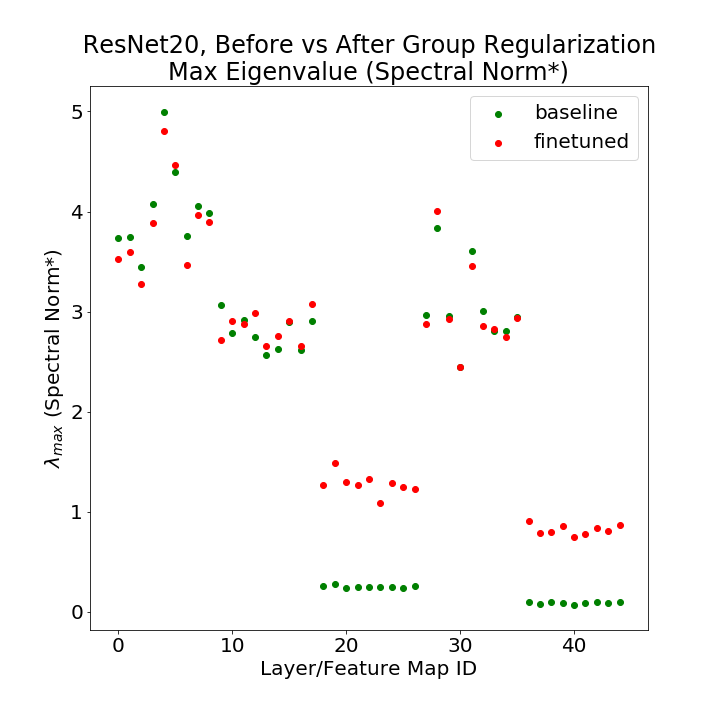
\includegraphics[width=4.5cm]{img/resnet4d_maxev.png}
      \label{fig:resnet204Dalpha}
   }
   \qquad
   \subfigure[$\alpha$ for ResNet20 layers]{
      %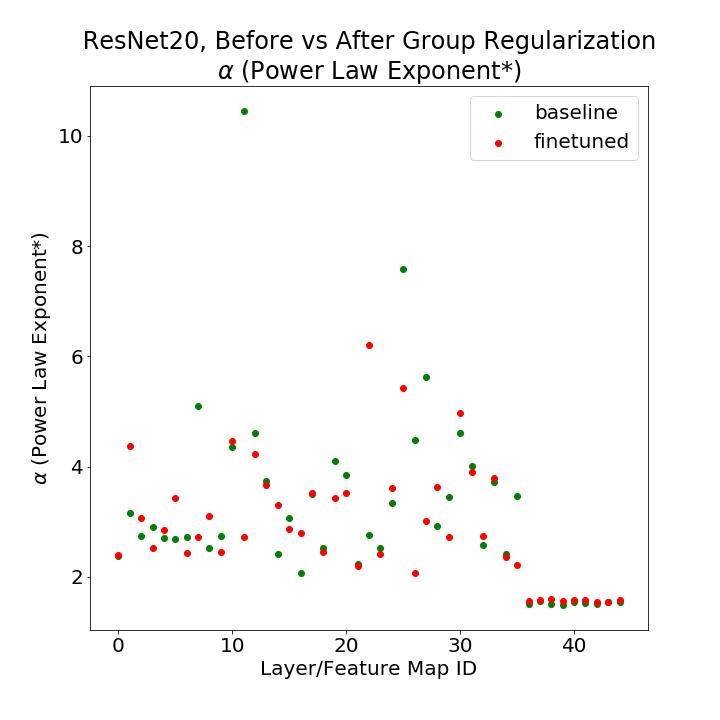
\includegraphics[scale=0.14]{img/resnet4d_alphas.png}
      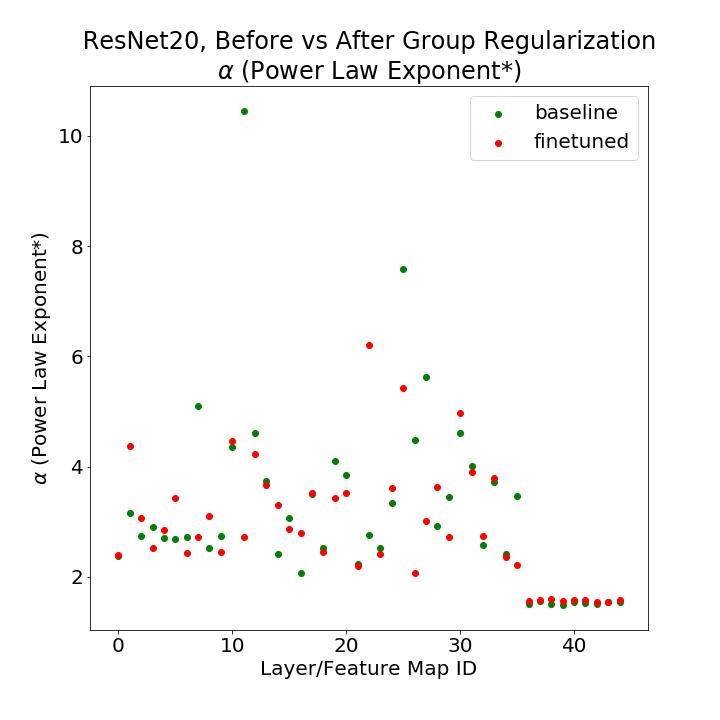
\includegraphics[width=3.7cm]{img/resnet4d_alphas.png}
      %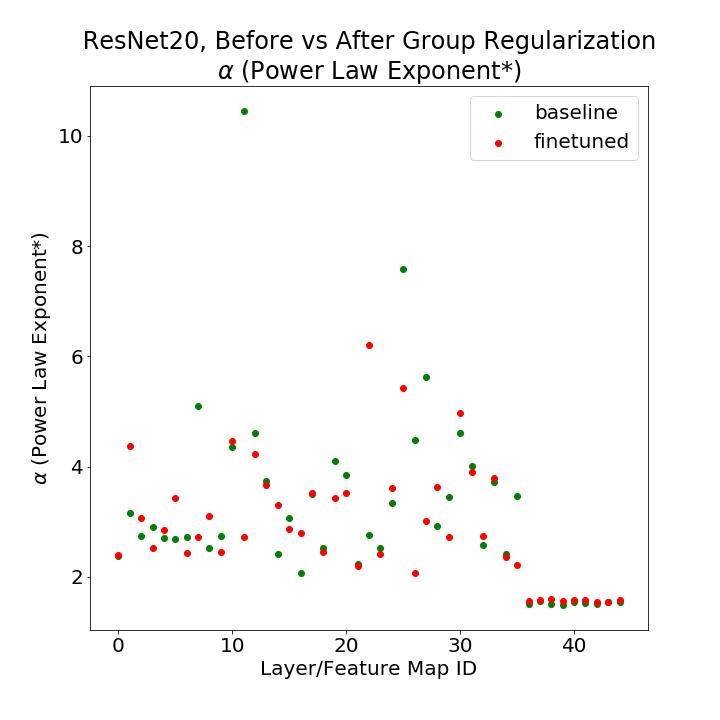
\includegraphics[width=4.5cm]{img/resnet4d_alphas.png}
      \label{fig:resnet204Dmaxev}
   }
   \caption{
     Analysis of ResNet20, distilled with Group Regularization, as implemented in the \texttt{distiller} (4D\_regularized\_5Lremoved) pre-trained models.  
     Comparison of individual layer $\mathbf{W}_{l}$ maximum eigenvalues ($\lambda_{max}$, or Spectral Norms) and  
     PL exponent $\alpha$, between baseline (green) and fine-tuned (red)  pre-trained models.   
           }
   \label{fig:resnet204D5L}
\end{figure}

Consider average metrics measured on ResNet20, trained on CIFAR10, before and after applying the Group Regularization technique, as implemented in the \texttt{distiller} package.%
\footnote{For details, see \url{https://nervanasystems.github.io/distiller/\#distiller-documentation} and also \url{https://github.com/NervanaSystems/distiller}.}
We analyze the available pre-trained 4D\_regularized\_5Lremoved baseline and fine-tuned models.  %\cite{distiller_repo}.
Figure~\ref{fig:resnet204D5L} presents the Spectral Norm ($\lambda_{max}$) and PL exponent ($\alpha$) for each individual layer weight matrix $\mathbf{W}_{l}$.%
\footnote{We only include layer matrices or feature maps with $M\ge50$.}
The reported baseline test accuracies ($Top1=91.450$ and $Top5=99.750$) are better than the reported fine-tuned test accuracies ($Top1=91.020$ and $Top5=99.670$).
Thus, the results of Figure~\ref{fig:vgg-metrics} and Figure~\ref{fig:cv2-accuracy} might suggest that the baseline Spectral (and Frobenius) Norm should be \emph{smaller} than those of the layers in the fine-tuned model.
In both cases (Frobenius norm results not shown), we observe the opposite.
On the other hand, the $\alpha$ values do not systematically differ between the baseline and fine-tuned models.
Also (not shown), the average (unweighted) baseline $\alpha$ is smaller than the fine-tuned average (as would be predicted by HT-SR Theory, on which $\hat{\alpha}$ is based).

The reason for this is that the \texttt{distiller} Group Regularization technique has the unusual effect of increasing the norms of the $\mathbf{W}$ feature maps for at least two of the Conv2D layers.
\michael{This impedance shuffling or whatever it is called messes up norms, but the strong correlations are still preserved, as seen in the $\hat{\alpha}$ metric, and the model quality is good.  CLARIFY.}


